\label{subsec:inputoutput}

Figure \ref{fig:interfaces} shows the messages exchanged at the interface of
the radio communication management module. The numbers in brackets represent the maximal value the message
may have. Note that in a first version the communication will only be set up
with an RBC, communication with a RIU (radio in-fill unit) are not taken
into account.

\begin{figure}[htpb]
\centering
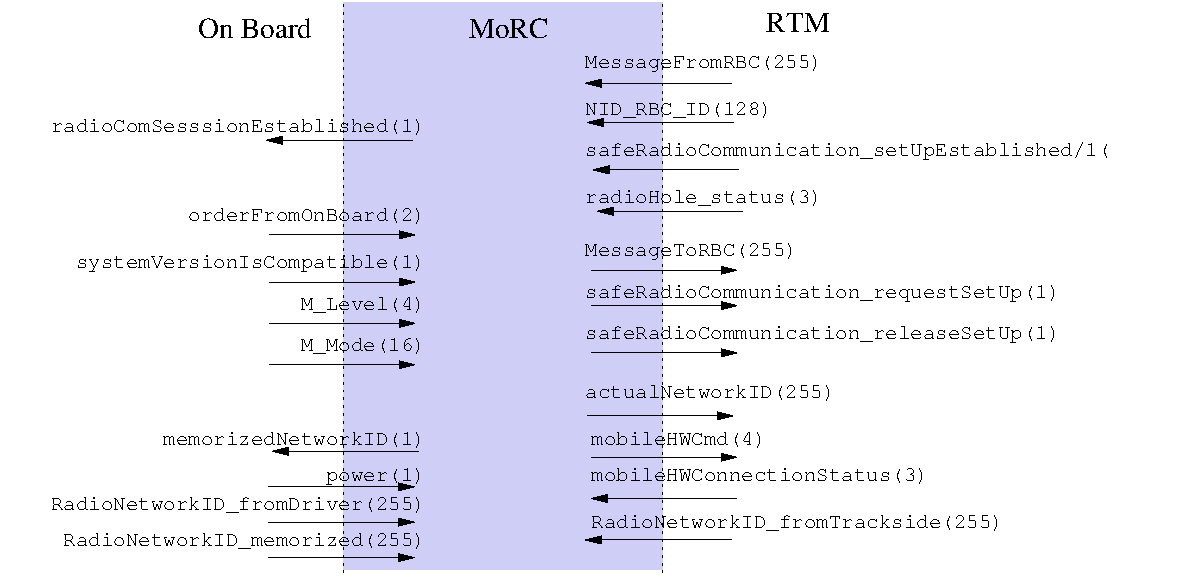
\includegraphics[width =.8\textwidth]{interface.pdf}
\caption{\label{fig:interfaces} Radio control manager interfaces.}
\end{figure}

\subsubsection{RTM interface}
\verb+MessageOut+, \verb+MessageIn+ are the Euroradio messages, their
possible values are defined in the subset-026-8.4 and the subset-026-7.4. The
test cases define by the subset-076 are performed by analyzing the recording of
these messages. In our model we have consider only the relevant messages.
Furthermore, messages are decomposed in variable and packets, these are not
taken into account by our modeling. Our model considers messages only as a number corresponding to an action. 
Table \ref{table:Messages} summarizes the considered messages, the message name
are those used in the model, Id and Packets are those defined in Subset-026-7
and Subset-026-8.

\begin{table}
  \caption{\label{table:Messages} Messages exchange during the Management of
  Radio Communication}
  \begin{tabular}{lclp{.4\textwidth}}\toprule
  Message Name & Id & Packets& Description \\\midrule
  \verb+TERM_SESSION_TRACK+& 24 & Packet 42 ; Q\_RBC = 0& The RBC orders the EVC to {\bf terminate} a communication with RBC \\
   \verb+INIT_SESSION_ORDER+ & 24 &Packet 42 ; Q\_RBC = 1 & 
   The RBC {\bf orders the initiation} of a communication \\
  \verb+SYS_VERSION+ & 32 & & The RBC {\bf acknowledge the initiation} of a
  communication and gives its system version \\
  \verb+INIT_SESSION_TRACK+ & 38 & &  The RBC {\bf initiates} a communication \\
  \verb+TERM_ACK+ & 39 & &  The RBC {\bf acknowledge} the termination of a communication \\
  \verb+TRANS_OVER_ORDER+ & 131 & & The RBC orders a {\bf transition order} over another RBC \\
  \verb+SYS_NO_COMP+ & 154 &&The EVC {\bf acknowledge the establishment with error}. \\
  \verb+INIT_SESSION+& 155 &&  The EVC {\bf initiates} a communication \\
  \verb+TERM_SESSION+ & 156&&The EVC {\bf terminates} a communication  \\
  \verb+SESSION_ESTABLISHED+ & 159 & & The EVC {\bf acknowledge the establishment} of a communication \\
  \verb+NO_MESSAGE+ & 255 & & No messages are send. \\
  \bottomrule
  \end{tabular}
\end{table}
\begin{description}
\item \verb+NID_Rbc+ identifies the RBC it joins the \verb+NID_RBC+ and
\verb+NID_C+ (Subset026-3).
\item \verb+setUp+,\verb+reqSetUp+,\verb+releaseSetUp+ messages are used for setting
or releasing a safe radio communication.
\item \verb+radioHole+ may have the value \verb+BEGIN+, \verb+INSIDE+,
\verb+END+ or
\verb+NONE+ regarding if the train enters, leaves or is in a announced radioHole 
are compatible.
\end{description}

\subsubsection{Interface with others on board functions}
The different cases to initiate or terminate a communication have been abstract
by a single signal. Since the behavior is the same regardless the different
events, we assume that others tasks of the EVC will activate the signal wen
needed.

\begin{description}
\item \verb+orderOnBoard+ represents the order from the on-board EVC to initiate
or terminate a communication. The possible values are the following ones~: 
  \begin{itemize}
  \item \verb+NONE+:  no order;
  \item \verb+INIT+ represents one of these cases :
	\begin{itemize}
	\item Start of mission procedure,
	\item Report a mode change,
	\item Driver change level to 2 or 3,
	\item End of a radio hole,
	\item The balise group orders a radio communication.
	\end{itemize}
  \item \verb+TERM+ represents one of these cases
	\begin{itemize}
	\item End of mission procedure, 
	\item Driver closes the desk,
	\item Error condition detected on-board.
	\item The balise group orders to end up a radio communication.
	\end{itemize}
  \end{itemize}
\item \verb+isCompatible+ is set to 1 if a the track and the on-board systems
(function system version management)
\end{description}

The radio management module should take some decision with respect to internal
on-board variables.
This variable are listed blow. The variable definition
are detailed in subset-026-7.
\begin{itemize}
\item \verb+M_LEVEL+ $\in [0..4]$ represents the levels 0,1,2,3 or NTC.
\item \verb+M_ mode+ $\in[0..15]$ represents the on-board operating mode
computed by mode function (SUBSET-026.4). 
\end{itemize}

% ----------------------------------------------------
\subsection{Internal variables}
\label{subsec:internalvar}


We define a set of variables use for the radio communication management
computation itself. Figure \ref{fig:Morc-class} shows the block element.
\begin{itemize}
\item \verb+countSetUp+, \verb+countMsg+, are used to count the number of try
for establishing a radio communication, or to wait for  the acknowledgment
message (SUBSET-026.3.A).
\item \verb+msgRecorded+: Keep track of \verb+MessageIn+
\item \verb+safeRadio+ $\in \{\mathtt{NOCOM, COM, LOST}\}$ indicates if a safe radio communication is on.
\item \verb+radoComSession+ $\in \{\mathtt{TERMINATED, ESTABLISHED}\}$: indicates if a radio session is established with the track.
\item \verb+time+ used for timeout evaluation
\end{itemize} 
Note that the \verb+safeRadio+ and \verb+radoComSession+ may be used for other
OBU functions like the messages given to the driver or mode computation

The constants or the enumeration type such as Modes name we had  used in the MorC
description are not part of the model itself, they should
belong to a special package.

\begin{figure}[htbp]
\centering
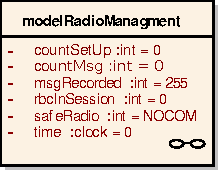
\includegraphics{MorC-class}
\caption{\label{fig:Morc-class} The MoRC class}
\end{figure}
